\section{Theoretical Background}

\subsection{Oscillators}

\subsubsection{Introduction to Oscillators}

\subsubsection{Collpits Oscillator}

\begin{figure}[!h]
    \centering
    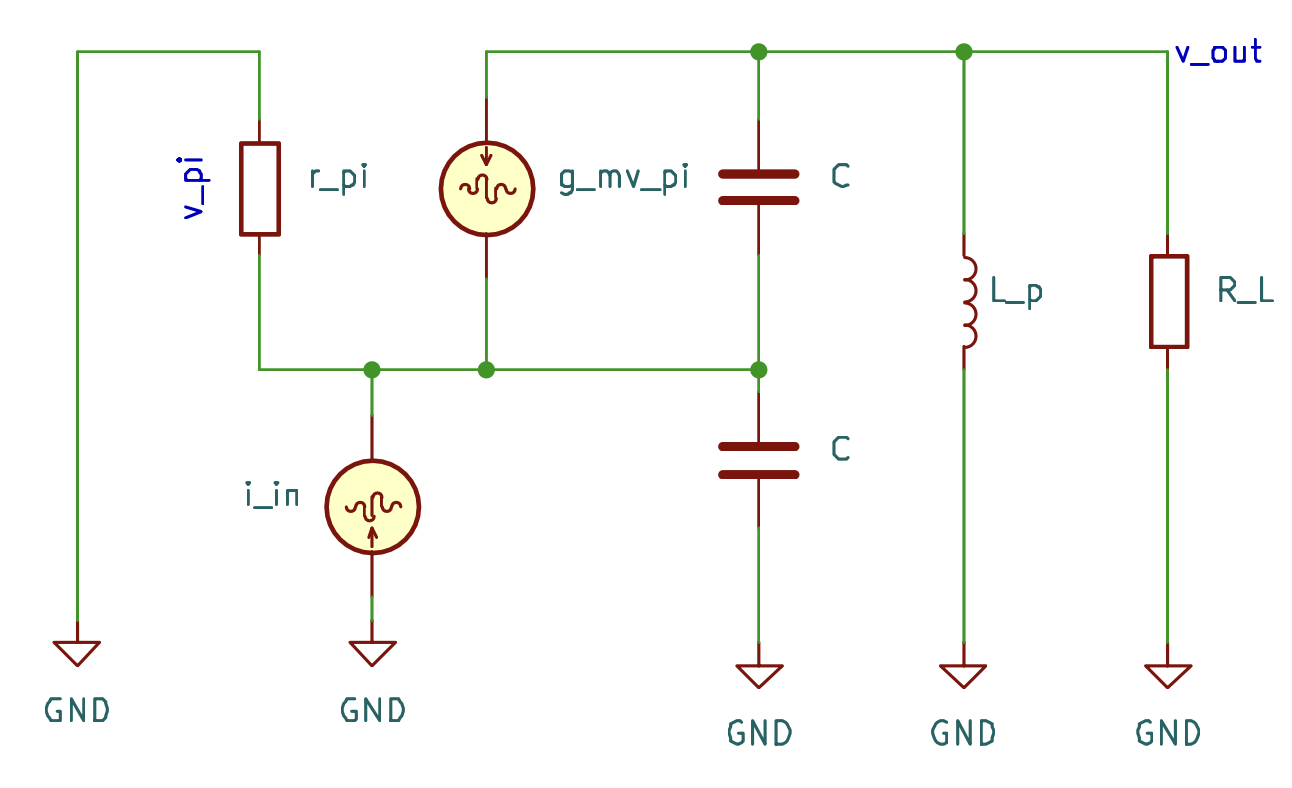
\includegraphics[width = 0.7\linewidth]{images/oscillator/design/ssm.png}
    \caption{Small Signal Model for Collpits Oscillator}
    \label{fig:ssm_collpits}
\end{figure}

We start with the given equations:
\begin{align}
    i_{in} &= -\frac{v_{\pi}}{r_{\pi}} - sC(v_{out} + 2v_{\pi}) \tag{1} \\
    0 &= g_mv_{\pi} + sC(v_{out} + v_{\pi}) + \frac{v_{out}}{sL_p} + \frac{v_{out}}{R_L}  \tag{2}
\end{align}

First, we simplify equation (2):
\begin{align*}
    g_mv_{\pi} + sCv_{out} + sCv_{\pi} + \frac{v_{out}}{sL_p} + \frac{v_{out}}{R_L} &= 0 \\
    g_mv_{\pi} + sCv_{\pi} + \left( sC + \frac{1}{sL_p} + \frac{1}{R_L} \right)v_{out} &= 0
\end{align*}

Solving for \(v_{\pi}\):
\begin{align*}
    v_{\pi}(g_m + sC) &= -\left( sC + \frac{1}{sL_p} + \frac{1}{R_L} \right)v_{out} \\
    v_{\pi} &= -\frac{\left( sC + \frac{1}{sL_p} + \frac{1}{R_L} \right)v_{out}}{g_m + sC}
\end{align*}

Substitute \(v_{\pi}\) back into equation (1):
\begin{align*}
    i_{in} &= -\frac{-\frac{\left( sC + \frac{1}{sL_p} + \frac{1}{R_L} \right)v_{out}}{g_m + sC}}{r_{\pi}} - sC\left( v_{out} + 2\left( -\frac{\left( sC + \frac{1}{sL_p} + \frac{1}{R_L} \right)v_{out}}{g_m + sC} \right) \right) \\
    &= \frac{\left( sC + \frac{1}{sL_p} + \frac{1}{R_L} \right)v_{out}}{r_{\pi}(g_m + sC)} - sCv_{out} - 2sC\left( -\frac{\left( sC + \frac{1}{sL_p} + \frac{1}{R_L} \right)v_{out}}{g_m + sC} \right) \\
    &= \frac{\left( sC + \frac{1}{sL_p} + \frac{1}{R_L} \right)v_{out}}{r_{\pi}(g_m + sC)} - sCv_{out} + \frac{2sC\left( sC + \frac{1}{sL_p} + \frac{1}{R_L} \right)v_{out}}{g_m + sC} \\
    &= v_{out} \left( \frac{\left( sC + \frac{1}{sL_p} + \frac{1}{R_L} \right)}{r_{\pi}(g_m + sC)} - sC + \frac{2sC\left( sC + \frac{1}{sL_p} + \frac{1}{R_L} \right)}{g_m + sC} \right)
\end{align*}

Combine the terms:
\begin{align*}
    i_{in} &= v_{out} \left( \frac{sC + \frac{1}{sL_p} + \frac{1}{R_L}}{r_{\pi}(g_m + sC)} - sC + \frac{2sC^2 + \frac{2sC}{sL_p} + \frac{2sC}{R_L}}{g_m + sC} \right)
\end{align*}

Since \(i_{in} = \frac{v_{out}}{Z_{in}}\), where \(Z_{in}\) is the input impedance:
\begin{align*}
    \frac{v_{out}}{i_{in}} &= Z_{in} \\
    &= \left( \frac{r_{\pi}C^2L_pR_Ls^3 + (-r_{\pi}CL_pR_Lg_m + 2r_{\pi}CL_p + CL_pR_L)s^2 + (2r_{\pi}CR_L + L_p)s + R_L}{r_{\pi}L_pR_Ls^3 + (-r_{\pi}CL_pR_Lg_m + 2r_{\pi}CL_p + CL_pR_L)s^2 + (2r_{\pi}CR_L + L_p)s + R_L} \right) \\
    &= r_{\pi}L_pR_L \left( s^2C + s g_m \right)
\end{align*}

Therefore, the frequency response is:
\begin{align}
    \frac{v_{out}}{i_{in}} &= \frac{r_{\pi}L_pR_L (s^2C + s g_m)}{r_{\pi}C^2L_pR_Ls^3 + (-r_{\pi}CL_pR_Lg_m + 2r_{\pi}CL_p + CL_pR_L)s^2 + (2r_{\pi}CR_L + L_p)s + R_L} \tag{3}
\end{align}
Put \(s = j\omega\) and let \(Im\) of denominator \(\to0\)
\begin{equation}
  \omega_0 = \sqrt{\frac{2r_\pi CR_L + L_p}{r_\pi C^2 L_p R_L}}
\end{equation}
Assuming \(r_\pi \to\infty\), as is the case is MOS, we reach the well-known expression \(\omega_0 = \sqrt{\frac{1}{L\frac{C.C}{C+C}}}\)

For sustained oscillations, we need
\begin{equation}
  -(-r_\pi C L_p R_L g_m + 2r_\pi C L_p + CL_p R_L)\omega^2_0 + R_L > 0
\end{equation}

This gives us
\begin{equation}\footnote{This is similar to the condition found in Razavi, but for NMOS in place of NPN BJT}
  R_L g_m -\frac{R_L}{r_\pi} -2 > 0
\end{equation}

Thus, we need to set \(R_L\) accordingly at the oscillating frequency, giving us a lower bound for load and thus a need for a matching network





\subsection{Matching Networks}


We assume a central impedance \(Z_c\) such that \(Z_c > \max(Z_s, Z_L)\), and then calculate the series and parallel reactive components on both sides.\footnote{In our case, all impedances are real}


\begin{minipage}[t]{0.48\textwidth}
\textbf{Source}:
\begin{equation}
    \begin{cases}
        \displaystyle Q_{src} = \sqrt{\frac{Z_c}{Z_s}-1}\\
        \displaystyle X_{src}^{parallel} = \frac{Z_c}{Q_{src}}\\
        \displaystyle X_{src}^{series} = Q_{src}Z_s
    \end{cases}
\end{equation}
\end{minipage}%
\hfill
\begin{minipage}[t]{0.48\textwidth}
\textbf{Load}:
\begin{equation}
    \begin{cases}
        \displaystyle Q_{ld} = \sqrt{\frac{Z_c}{Z_L}-1}\\
        \displaystyle X_{ld}^{parallel} = \frac{Z_c}{Q_{ld}}\\
        \displaystyle X_{ld}^{series} = Q_{ld}Z_L
    \end{cases}
\end{equation}
\end{minipage}

\[L=\frac{X}{2\pi f_0} \quad \text{and} \quad C = \frac{1}{2\pi f_0 X}\]
for chosen \(X\) series/parallel

After this, the values of \(V_{cc}, V_{ee}, \) and \(I_c\) were changed so as to get the maximum efficiency. \(R_L\) was matched to \(1[K\Omega]\).

\begin{table}[!h]
\centering
\begin{tabular}{|c|c|}
    \hline
    \textbf{Variable} & \textbf{Value} \\
    \hline
    $f_0$ & $3.5 \times 10^9$ \\
    $Z_{\text{out\_osc}}$ & $1000$ \\
    $Z_{\text{load}}$ & $50$ \\
    $Z_{\text{center}}$ & $1002$ \\
    $Q_{\text{src}}$ & $0.0447214$ \\
    $X_{\text{paralle\_src}}$ & $22405.4$ \\
    $X_{\text{series\_src}}$ & $44.7214$ \\
    $L_{\text{src}}$ & $2.03361 \times 10^{-9}$ \\
    \hline
\end{tabular}
\end{table} 
\begin{table}[!h]
\centering
\begin{tabular}{|c|c|}
    \hline
    \textbf{Variable} & \textbf{Value} \\
    \hline
    $C_{\text{src}}$ & $2.02955 \times 10^{-15}$ \\
    $Q_{\text{ld}}$ & $4.36348$ \\
    $X_{\text{paralle\_ld}}$ & $229.633$ \\
    $X_{\text{series\_ld}}$ & $218.174$ \\
    $L_{\text{ld}}$ & $1.04421 \times 10^{-8}$ \\
    $C_{\text{ld}}$ & $2.08424 \times 10^{-13}$ \\
    $C_{\text{com}}$ & $2.10454 \times 10^{-13}$ \\
    $L_{\text{com}}$ & $1.70212 \times 10^{-9}$ \\
    \hline
\end{tabular}
\end{table} 

\subsection{Antenna}